\chapter{Použití teoretických poznatků}\label{chap:praxe}
Tato kapitola přímo vychází z teorie vysvětlené v kapitole \ref{kap:teorie} a snaží se ji využít při návrhu větrné turbíny.

\section{Parametry návrhu}
V této podkapitole bych rád vytyčil cíle, respektive požadované parametry, navrhované větrné turbíny.

Jak jsem již zmínil v úvodu, čím menší větrná turbína, tím méně je ekonomicky rentabilní. Turbíny s průměrem menším než 5~metrů jsou v podstatě nerentabilní. Proto se v návrhu nebudu omezovat komplikovaností či finanční náročností výroby turbíny. Cílem je navrhnout co nejúčinnější turbínu, která může být umístěna v zástavbě a bude fungovat jako technická zajímavost.

Jelikož bude turbína umístěna v zástavbě, je nutné zvolit rozumnou velikost, aby nebyla příliš rušivá. Čím větší turbína, tím jsou také nižší otáčky při stejné rychloběžnosti. S velkou turbínou se také pojí vyšší zatížení stožáru, který pak musí být kotven např. pomocí lan, což je v zástavbě, resp. na zahrádce, značně omezující. Naopak i malý přírůstek na průměru přidá na výkonu turbíny – výkon turbíny je odvislý od její plochy, přičemž ta roste se čtvercem poloměru. Nakonec jsem se rozhodl pro návrh turbíny s průměrem 2,5~m. Vycházel jsem zde ze zkušeností s~prvním prototypem, jehož průměr 1,5~metru se ukázal jako malý a průměr turbíny přes 3~metry by mohl působit značně rušivě. Navíc již nyní se vyskytly problémy s~manipulací se sestavenou 1,5m turbínou.

Dalším charakteristickým znakem větrné turbíny je počet listů. Zde jsem zvolil 3. Toto číslo bylo zvoleno adekvátně k požadované rychloběžnosti dle tabulky na straně 70 v knize \cite{Rychetnik:Motory}. Navíc vzhled turbíny je „přirozený“ – většině lidí se pod pojmem větrná elektrárna vybaví právě třílistá turbína.

Posledním voleným parametrem turbíny je její rychloběžnost. U prvního prototypu byla zvolena relativně nízká rychloběžnost~4 díky obavám z hluku (při vyšší rychloběžnosti se konce listů pochybují rychle, čímž snadněji vyvolávají hluk). Obavy se ukázaly jako neopodstatněné. Podle grafu na stránkách \cite{ve:ve}\footnote{http://ve.ic.cz/files/teorie/ucinnost.png}  a tabulky 3.1 v knize \cite{Rychetnik:Motory}, leží maximální účinnost třílisté turbíny mezi rychloběžností 5 a 6. Jelikož požadavek na nízkou hlučnost je relativně důležitý, rozhodl jsem se pro jistotu zvolit rychloběžnost 5.

Jelikož není potřeba vytvářet síťové napětí, nebude mít turbína z důvodu jednoduchosti nastavitelné listy pro regulaci otáček. Tím se také zvýší její účinnost.

\section{Výběr profilu}
Prvním krokem při návrhu turbíny hned po stanovení jejích parametrů je výběr turbíny. Z~předchozí teorie vypadá, že stačí vybrat pouze profil s co největším poměrem součinitelů $c_y/c_x$. Výběr profilu však má některá úskalí, která bych v této kapitole chtěl probrat.

\subsection{Reynoldsovo číslo}
V kapitole \ref{kap:zakladprinc} jsem zmínil, že aerodynamické vlastnosti profilu souvisí s podmínkami, ve kterým je provozován. Tyto podmínky charakterizuje Reynoldsdovo číslo \cite{Rychetnik:Motory}, která bylo definováno v rovnici \eqref{rov:13}.

Jedná se pouze o orientační údaj; vlastnosti profilů se na jeho velikosti mění pouze málo. Např. pro profil SG6043 je součinitel $c_y$ pro $Re$ $10^5$ roven 1,415; pro $7,5\cdot 10^4$ 1,408 a pro $5\cdot 10^4$ je 1,389. Tato data byla převzata z \cite{profil}\footnote{http://www.worldofkrauss.com/foils/getpolar/787.dat}. Navíc parametry profilů jsou dostupné pouze pro některá Re.
Abych mohl spočítat $Re$, je nutné odhadnout délku tětivy. Její délka se však výrazně mění. Většinou se však uvažuje délka tětivy u konce listu, která má největší podíl na výkonu. Délka tětivy se v tomto případě pohybuje okolo 10~cm.

Také rychlost obtékání profilu se uvažuje pouze jako obvodová rychlost rotoru, nikoliv jako vektorový součin obvodové rychlosti rotoru a rychlosti větru. Pro vítr o rychlosti 4 $m\cdot s^{-1}$ je~$Re$ \eqref{rov:50}:
\begin{equation}
	\label{rov:50}
	Re=\frac{vl}{\nu}=\frac{v_1\cdot\lambda l}{\nu}=\frac{4\cdot 5 \cdot 0,1}{15\cdot 10^6}\doteq 1,33\cdot 10^5
	\end{equation}
Je tedy nutné vybírat z profilů, které vykazují dobré vlastnosti při $Re$ $1,33\cdot 10^5$.

\subsection{Ideální vlastnosti profilu}
V~tabulkách k~daným profilům, lze zpravidla najít údaj o maximální hodnotě poměru $c_y/c_x$ (též označovaného jako jemnost profilu). Z~čistě teoretického hlediska lze říci, že tento parametr je dostačující.

V praxi však nelze dosáhnout ideálních podmínek. Všechny teorie uvedené v předchozí kapitole předpokládají, že směr relativní rychlosti větru $\beta$ je konstantní. V praxi to však nelze dodržet. Zpravidla nastávají tři nepříznivé situace:
\paragraph{Vítr nevane v celé ploše turbíny stejnou rychlostí.} Tento jev se projevuje hlavně u~velkých turbín. Avšak má vliv i na malé turbíny, zejména v turbulentním prostředí, kde jsou rozdíly rychlostí velké. Zástavba takovým prostředím bezpochyby je.
\paragraph{Turbína je zatížena.} Při přílišném zatížení turbíny se sníží její rychlost otáčení, což vede ke snížení rychloběžnosti a změně směru relativní rychlosti větru.
\paragraph{Turbína se rozbíhá.} Při rozběhu se turbína otáčí pomaleji než je navržena, tudíž její rychloběžnost opět není konstantní a relativní proud vzduchu má opět jiný směr než ideální.\vspace{0.5cm}

Z těchto důvodů je vhodné, aby profil měl co nejpodobnější hodnoty součinitelů $c_x$ a $c_y$ pro co největší rozsah úhlů náběhu – díky tomu bude turbína podávat dobré vlastnosti i při nepříznivých podmínkách. Je také výhodné, aby maximální hodnota jemnosti profilu měla podobné hodnoty od sebe jak v~kladném, tak i záporném směru – důvod je zřejmý. Na grafech \ref{graf.jemnost1}, \ref{graf:jemnost2} a \ref{graf:jemnost3} jsou zobrazeny ilustrační příklady takových průběhů jemnosti profilu.

\begin{figure}[H]
	\centering
	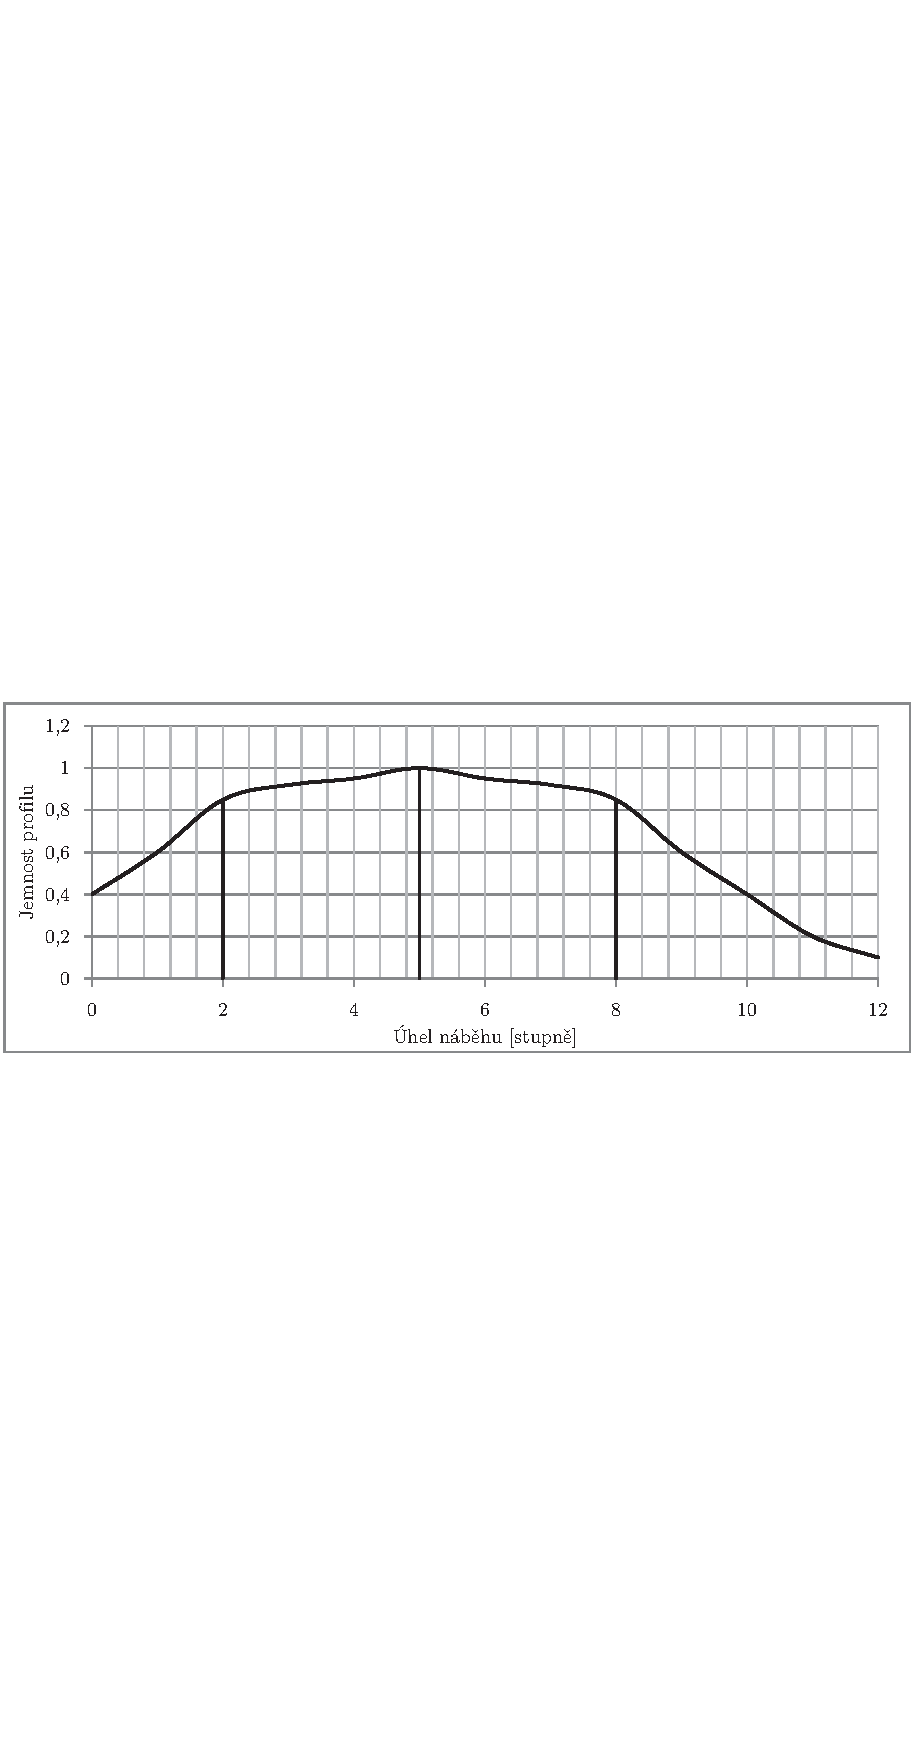
\includegraphics[]{obrazky/grafy/jemnost1p}
	\caption{Graf zobrazuje vhodný průběh jemnosti profilu k úhlu náběhu. Je vidět, že profil dává v~rozmězí $2$–$8\,^{\circ}$ velmi podobné výsledky. Data jsou pouze ilustrační, nejsou založena na žádném existujícím profilu}
	\label{graf.jemnost1}
\end{figure}

	\begin{figure}[H]
	\centering
	\subfigure[Maximálních hodnot jemnosti profil dosahuje pouze na minimálním úseku]{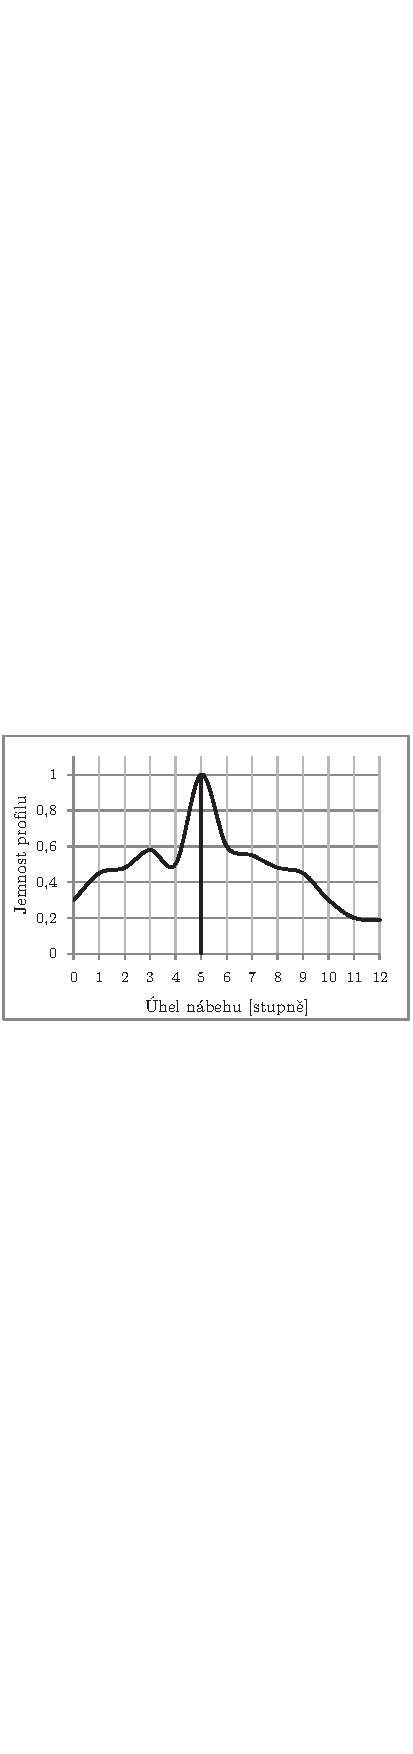
\includegraphics[]{obrazky/grafy/jemnost2p}\label{graf:jemnost2}}~
	\subfigure[Charakteristika je výrazně asymetrická]{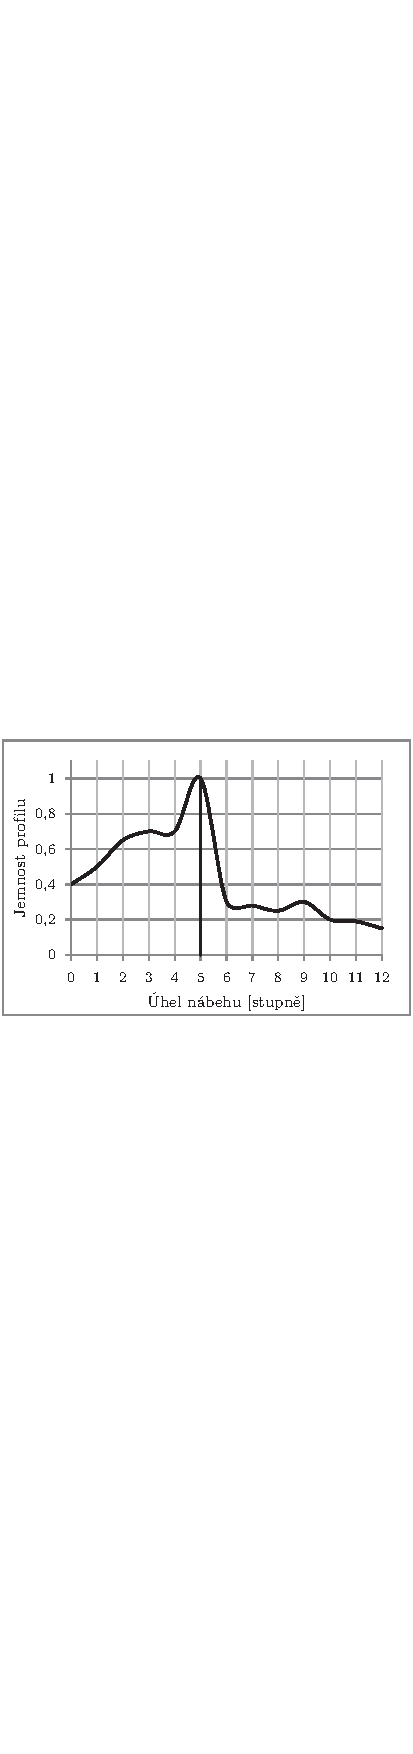
\includegraphics[]{obrazky/grafy/jemnost3p}\label{graf:jemnost3}}
	\caption{Grafy znázorňují nevhodný průběh jemnosti profilu. Data jsou pouze ilustrační.}
	\end{figure}
	
\subsection{Výběr profilu}
	Ze stránek Airfoil Inverstigation Database \cite{profil} jsem vybral několik na první pohled vhodných profilů. A to profily WORTMANN FX 60-126, EPPLER 395, GOE 481A a SG6043. V této kapitole je na základě výše uvedených kritérií porovnám. Veškerá data o profilech jsou převzata také z těchto stránek.
	\paragraph{WORTMANN FX 60-126}(obrázek \ref{profil:wort}) Tento profil na první pohled zaujme vysokou jemností profilu (graf \ref{profil:wortj}) – 170 při úhlu náběhu $5\,^{\circ}$. Avšak při pohled na průběh jemnosti je jasné, že tento profil není vhodný do nepříznivých podmínek – ideálních hodnot dosahuje pouze na malém intervalu úhlů náběhu, navíc asymetricky.
	\begin{figure}[H]
		\centering
		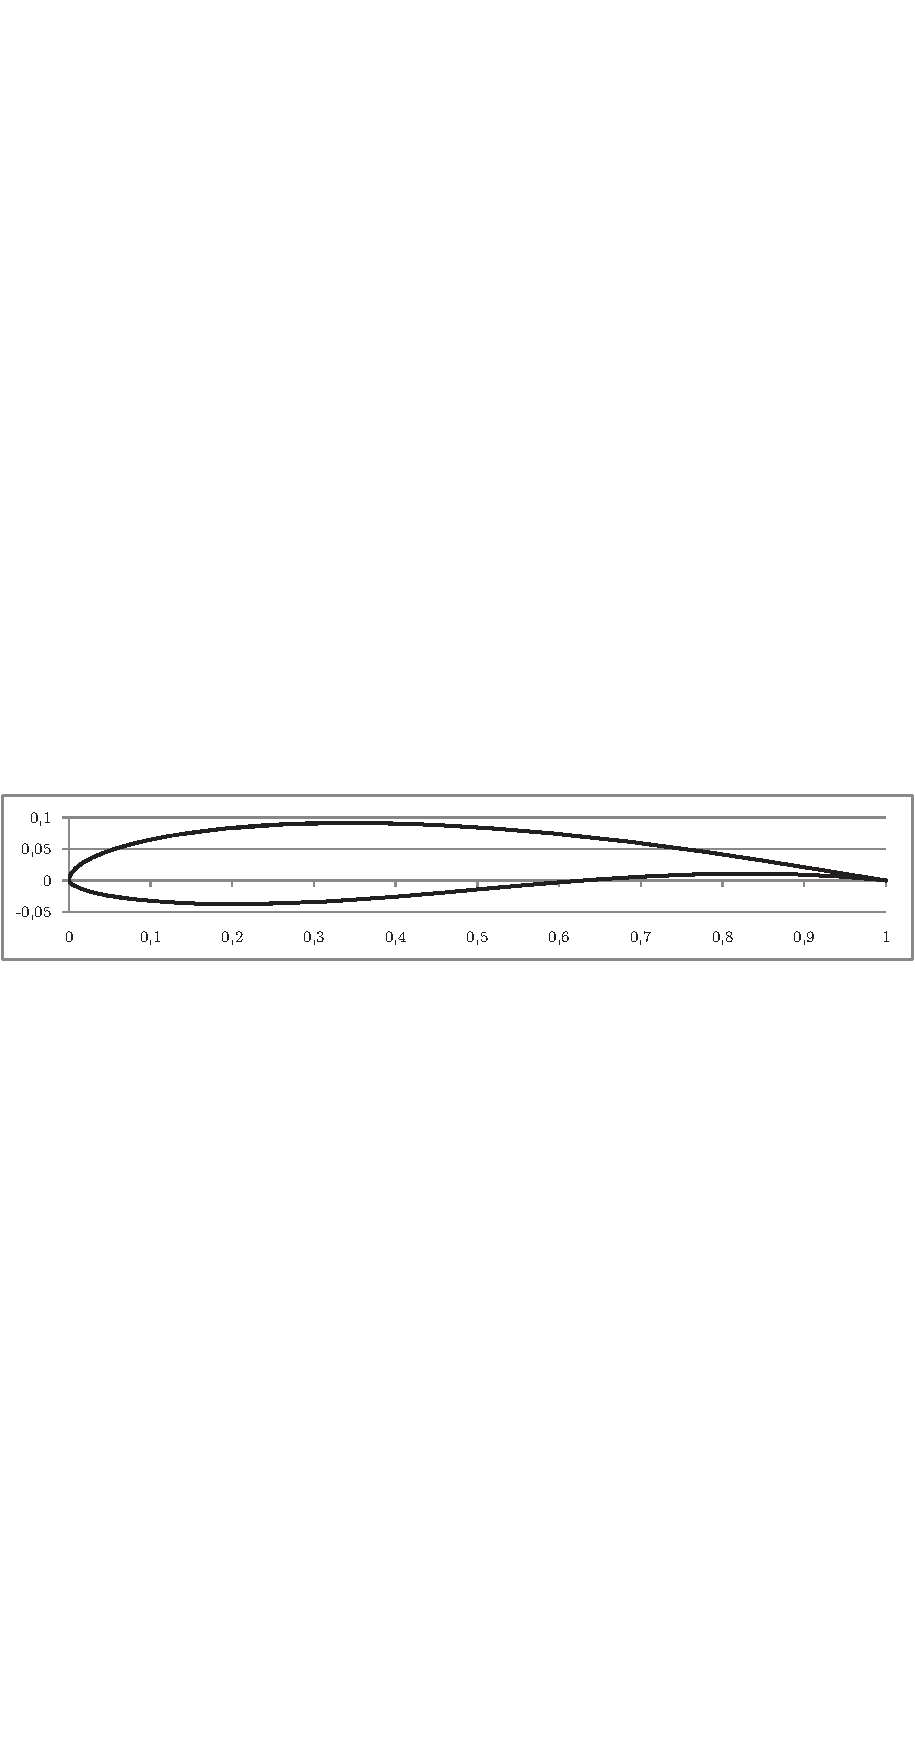
\includegraphics[]{obrazky/grafy/wortmannp}
		\caption{Profil WORTMANN FX 60-126}
		\label{profil:wort}
	\end{figure}
	\begin{figure}[H]
			\centering
			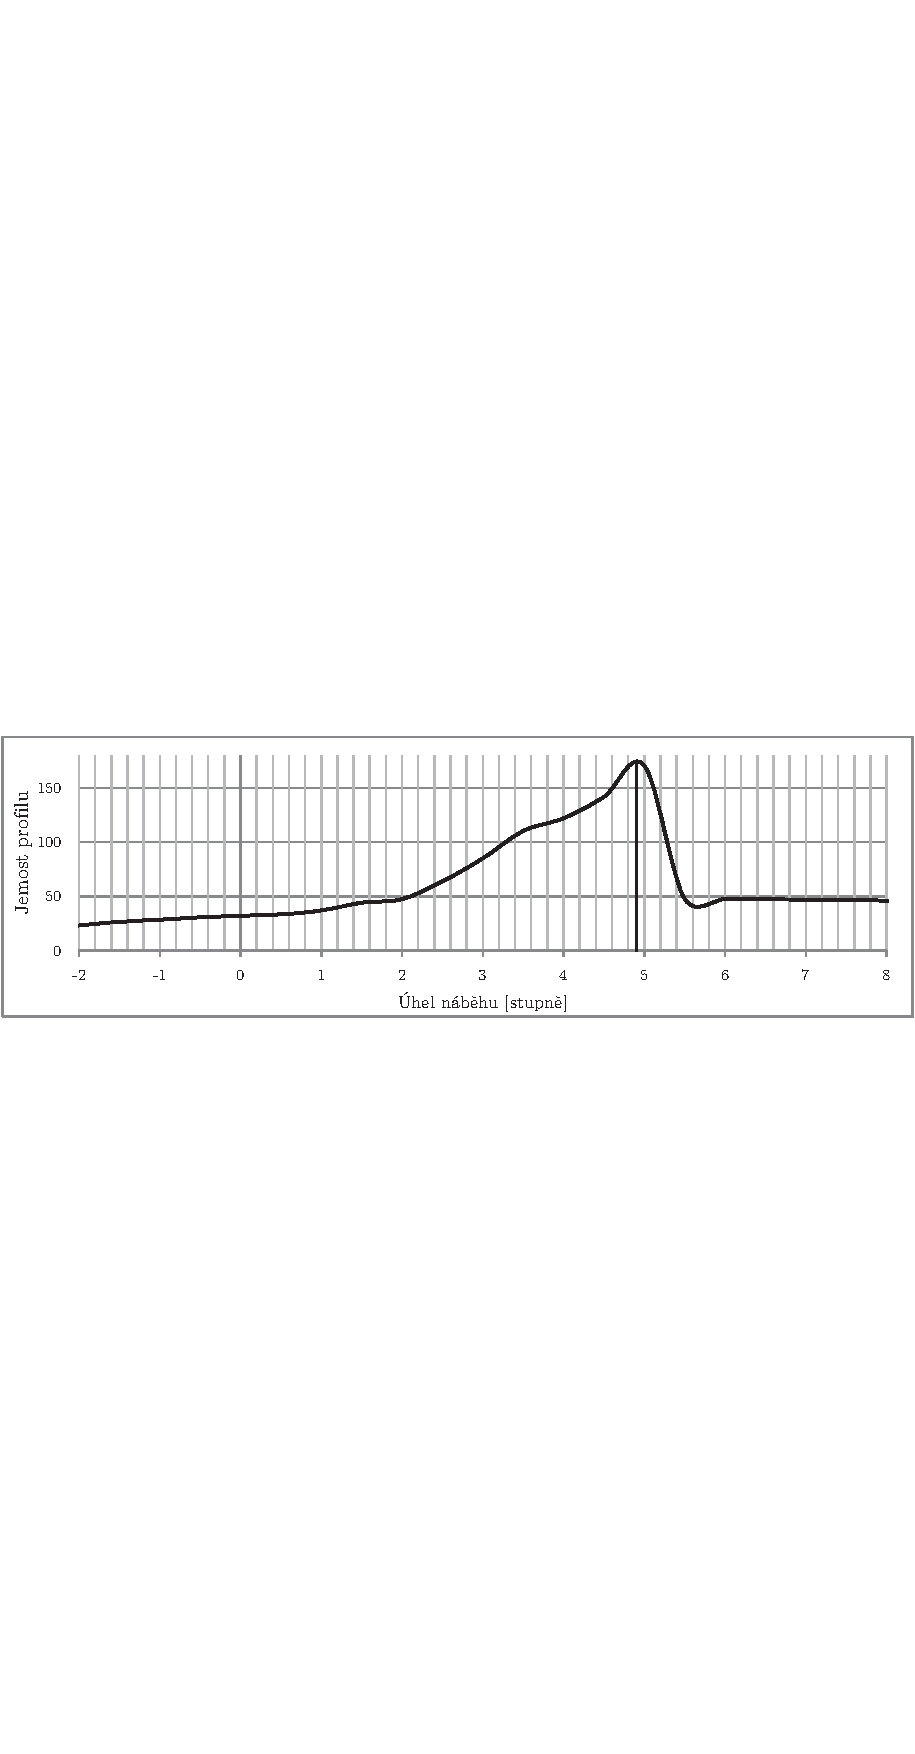
\includegraphics[]{obrazky/grafy/wortmannjp}
			\caption{Jemnost profilu WORTMANN FX 60-126}
			\label{profil:wortj}
	\end{figure}
	\paragraph{EPPLER 395} (obrázek \ref{profil:epp}) Tento profil opět na první pohled lákal vysou jemností (graf \ref{profil:eppj}) – 80. Směrem do záporných hodnot jeho jemnost klesá pozvolna, avšak do kladných prudce klesá. Pro mé podmínky se jedná o nevhodný profil.
	\begin{figure}[H]
			\centering
			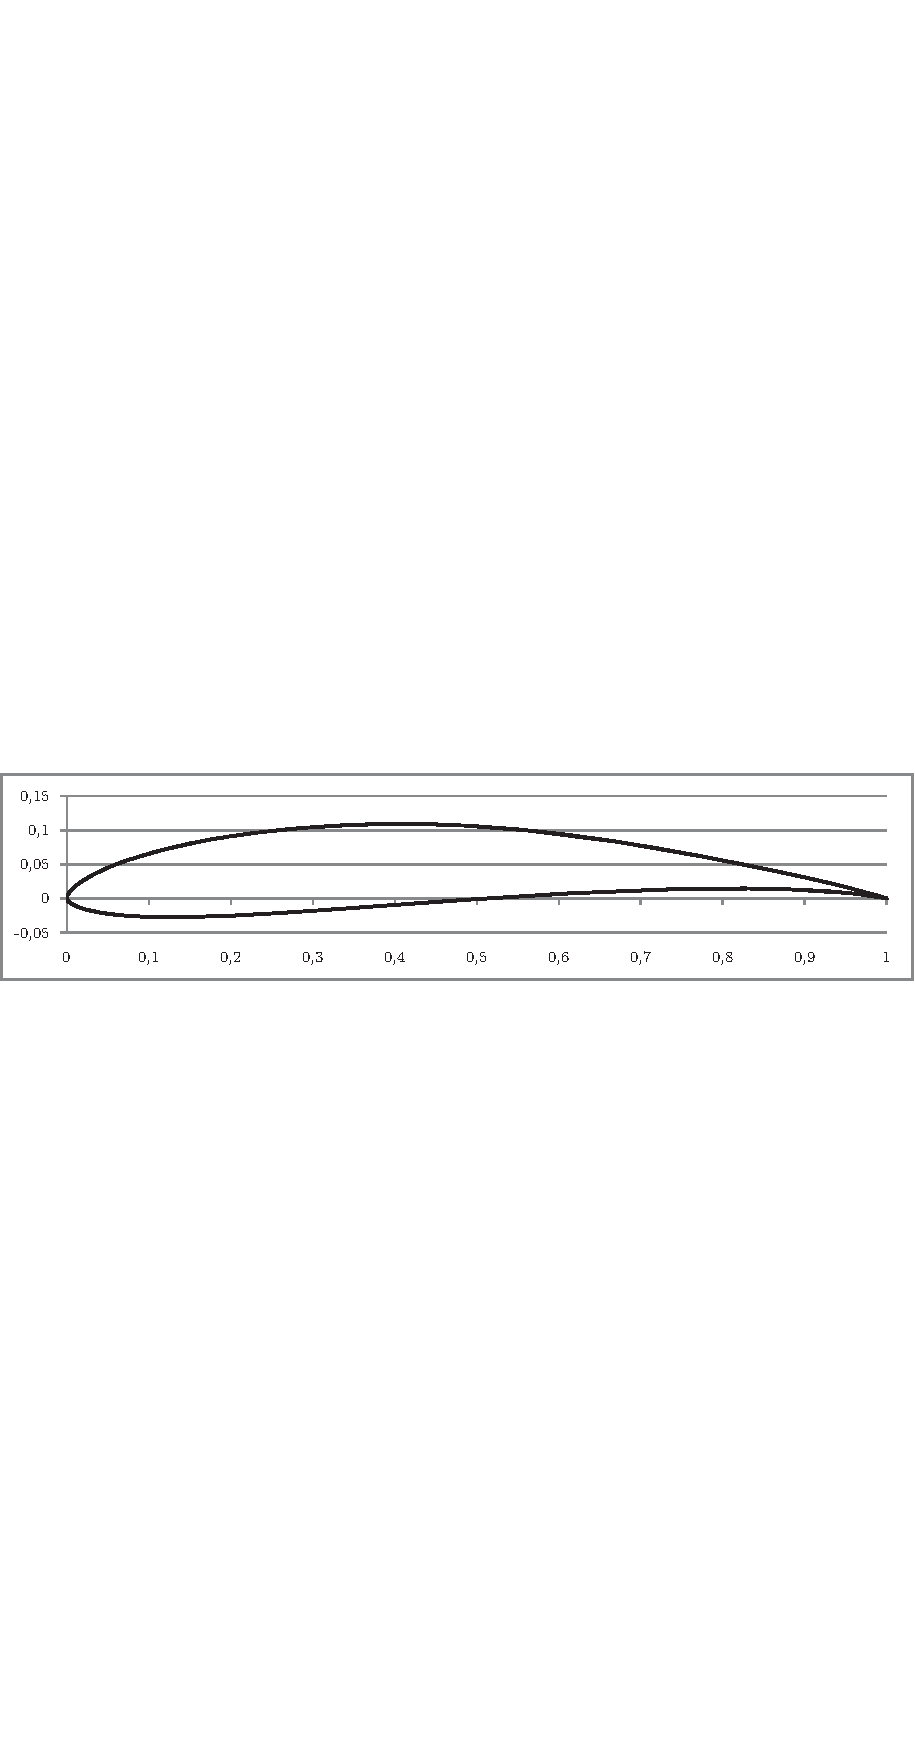
\includegraphics[]{obrazky/grafy/eppp}
			\caption{Profil EPPLER 395}
			\label{profil:epp}
		\end{figure}
		\begin{figure}[H]
				\centering
				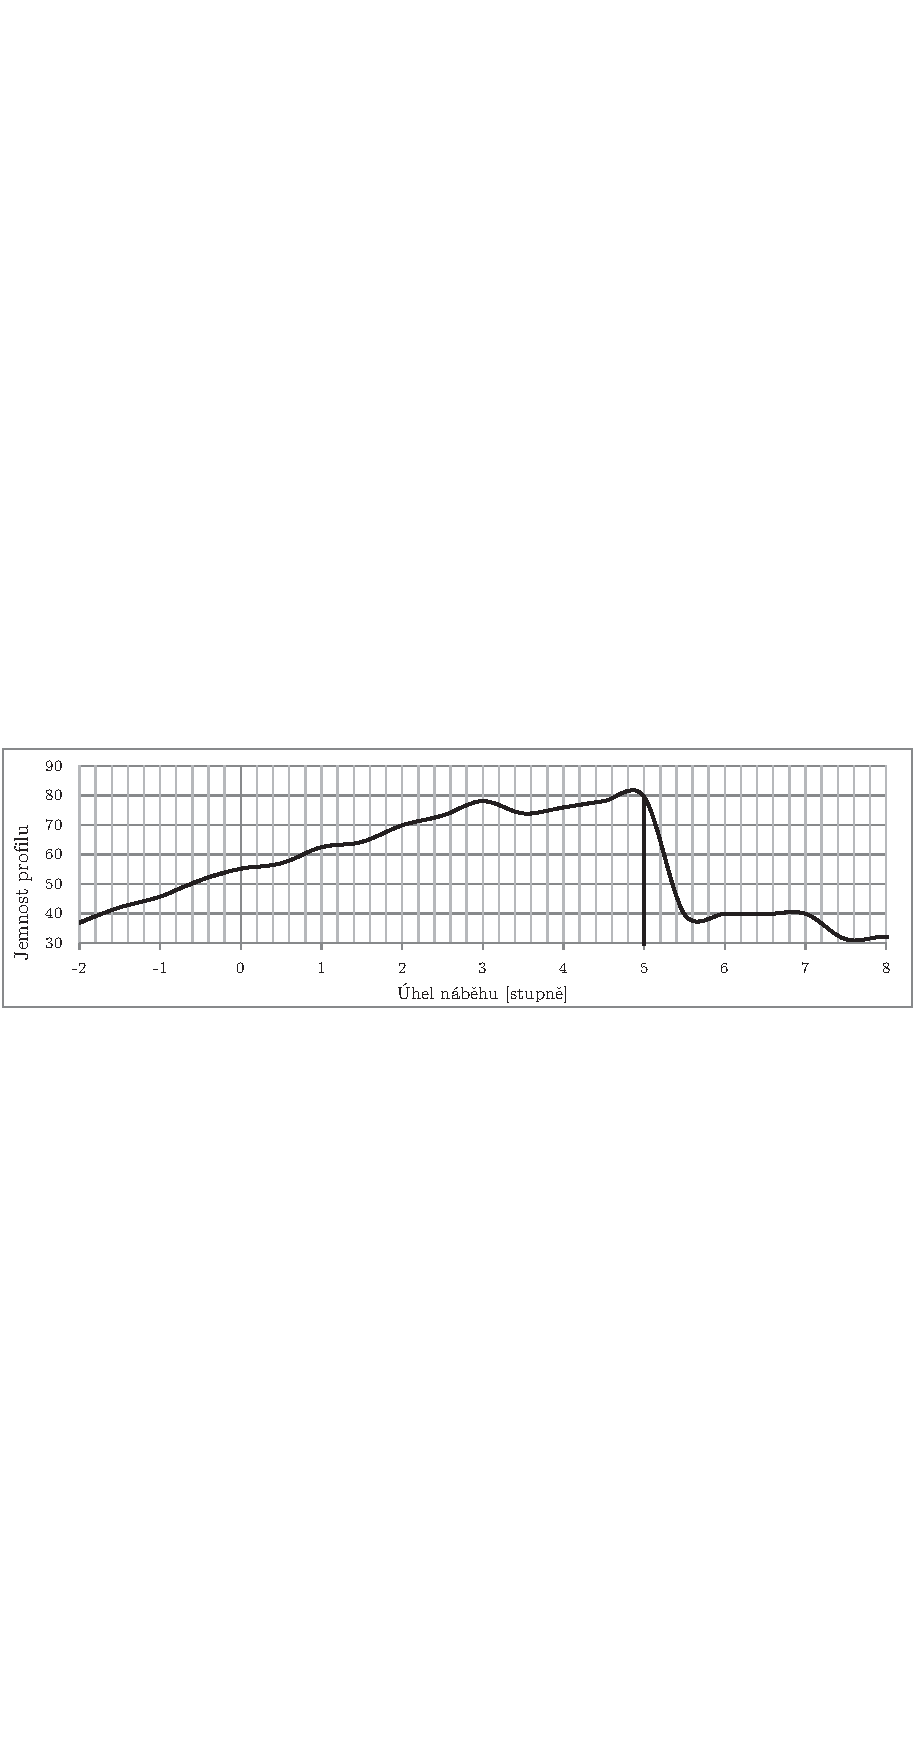
\includegraphics[]{obrazky/grafy/eppjp}
				\caption{Jemnost profilu EPPLER 395}
				\label{profil:eppj}
		\end{figure}
	\paragraph{GOE481A} (obrázek \ref{profil:goe}) Tento profil dosahuje jemnosti 73 a tuto vysokou jemnost udržuje na dlouhém intervalu úhlů náběhu – od 3 do $8\,^{\circ}$ (graf \ref{profil:goej}). Má i relativně velkou tloušťku, což je výhodné pro konstrukci listu.
	\begin{figure}[H]
			\centering
			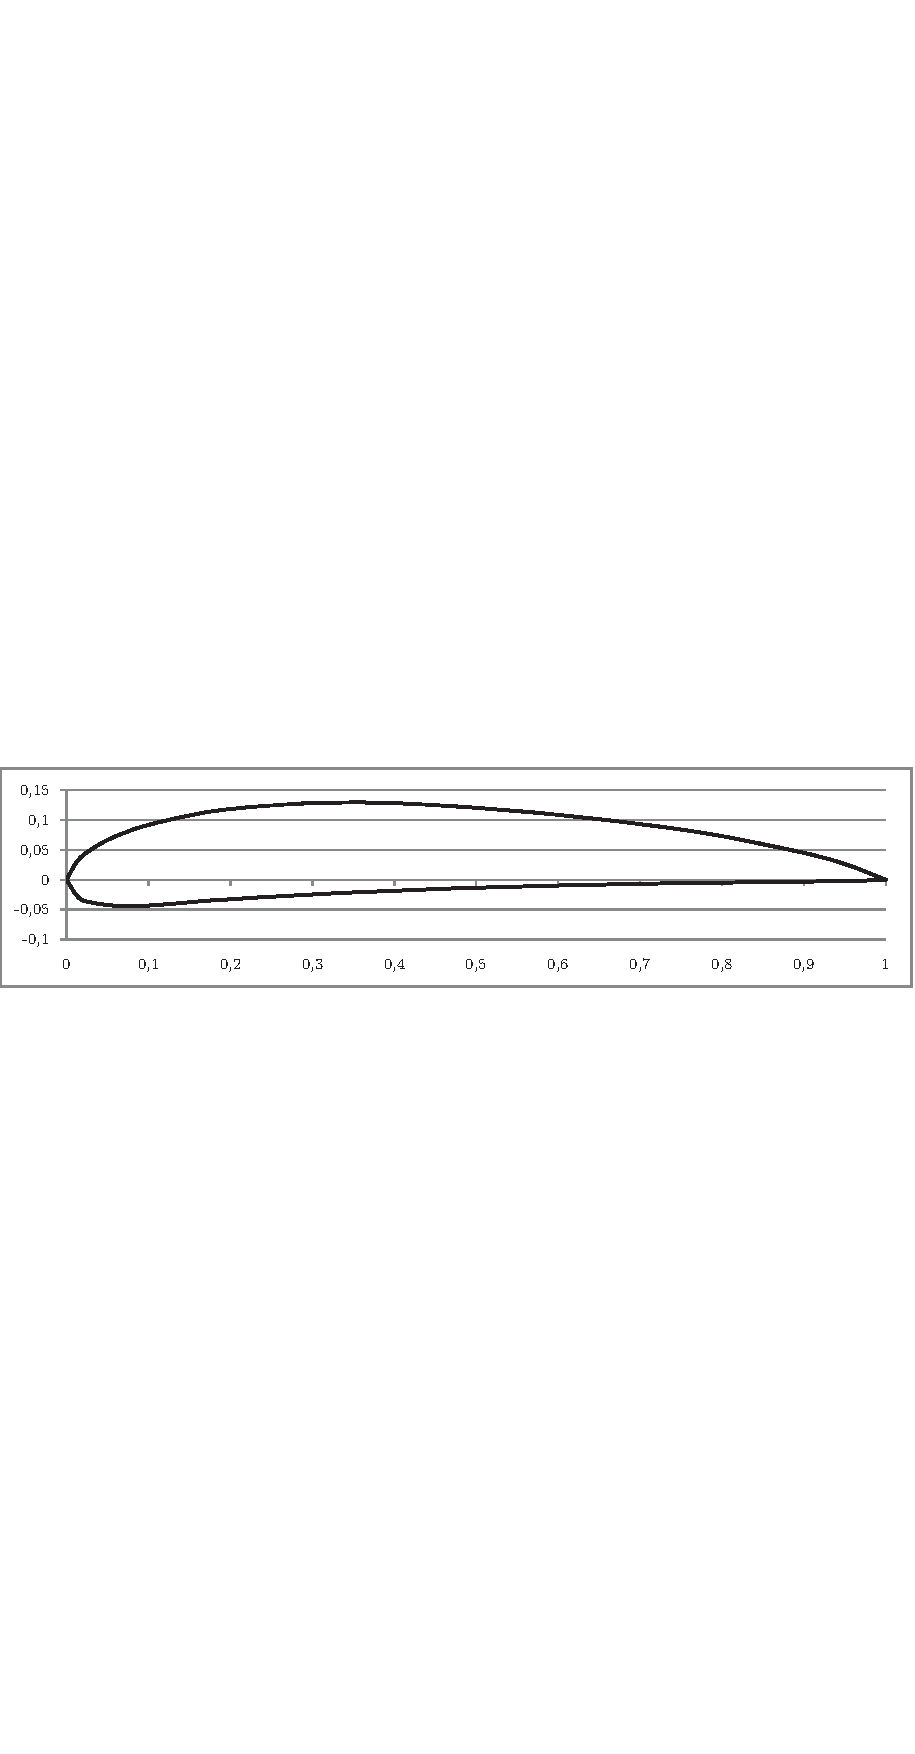
\includegraphics[]{obrazky/grafy/goep}
			\caption{Profil GOE481A}
			\label{profil:goe}
		\end{figure}
		\begin{figure}[H]
				\centering
				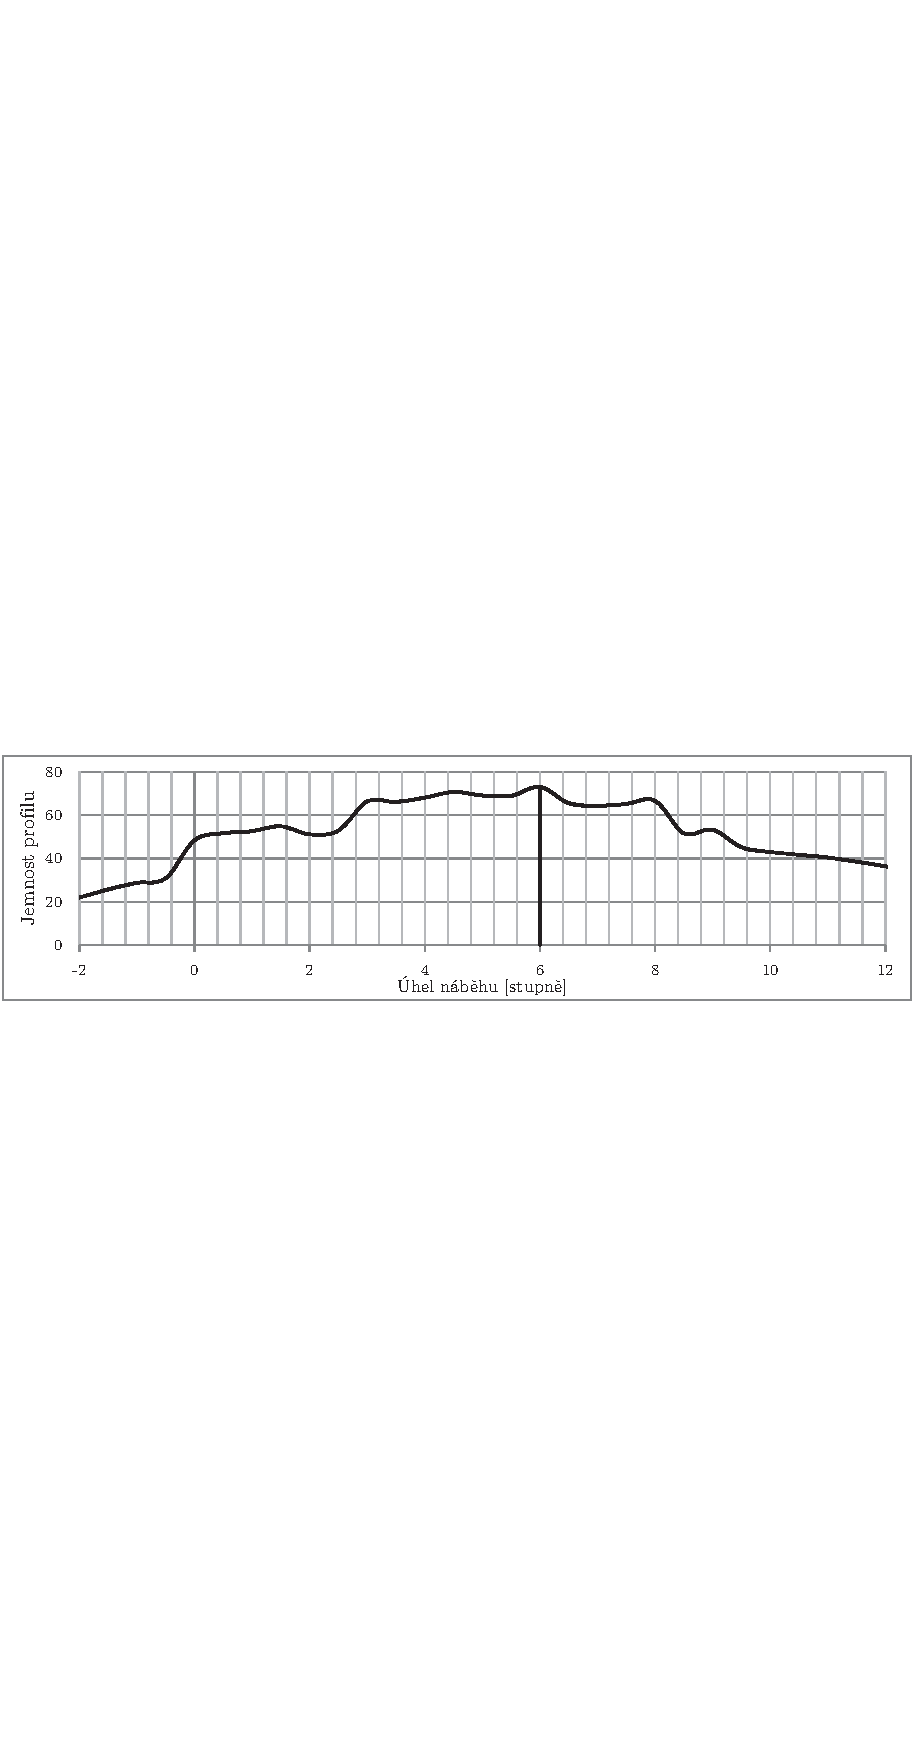
\includegraphics[]{obrazky/grafy/goejp}
				\caption{Jemnost profilu GOE481A}
				\label{profil:goej}
		\end{figure}
		
	\paragraph{SG6043} (obrázek \ref{profil:sg}) Tento profil podobně jako GOE481A dosahuje jemnosti 70 a drží si ji na podobném intervalu (graf \ref{profil:sgj}). Oproti němu však tyto hodnoty nekolísají, což je výhodné. Jeho nevýhodou v porovnání s GOE481A je menší tloušťka.
		\begin{figure}[H]
				\centering
				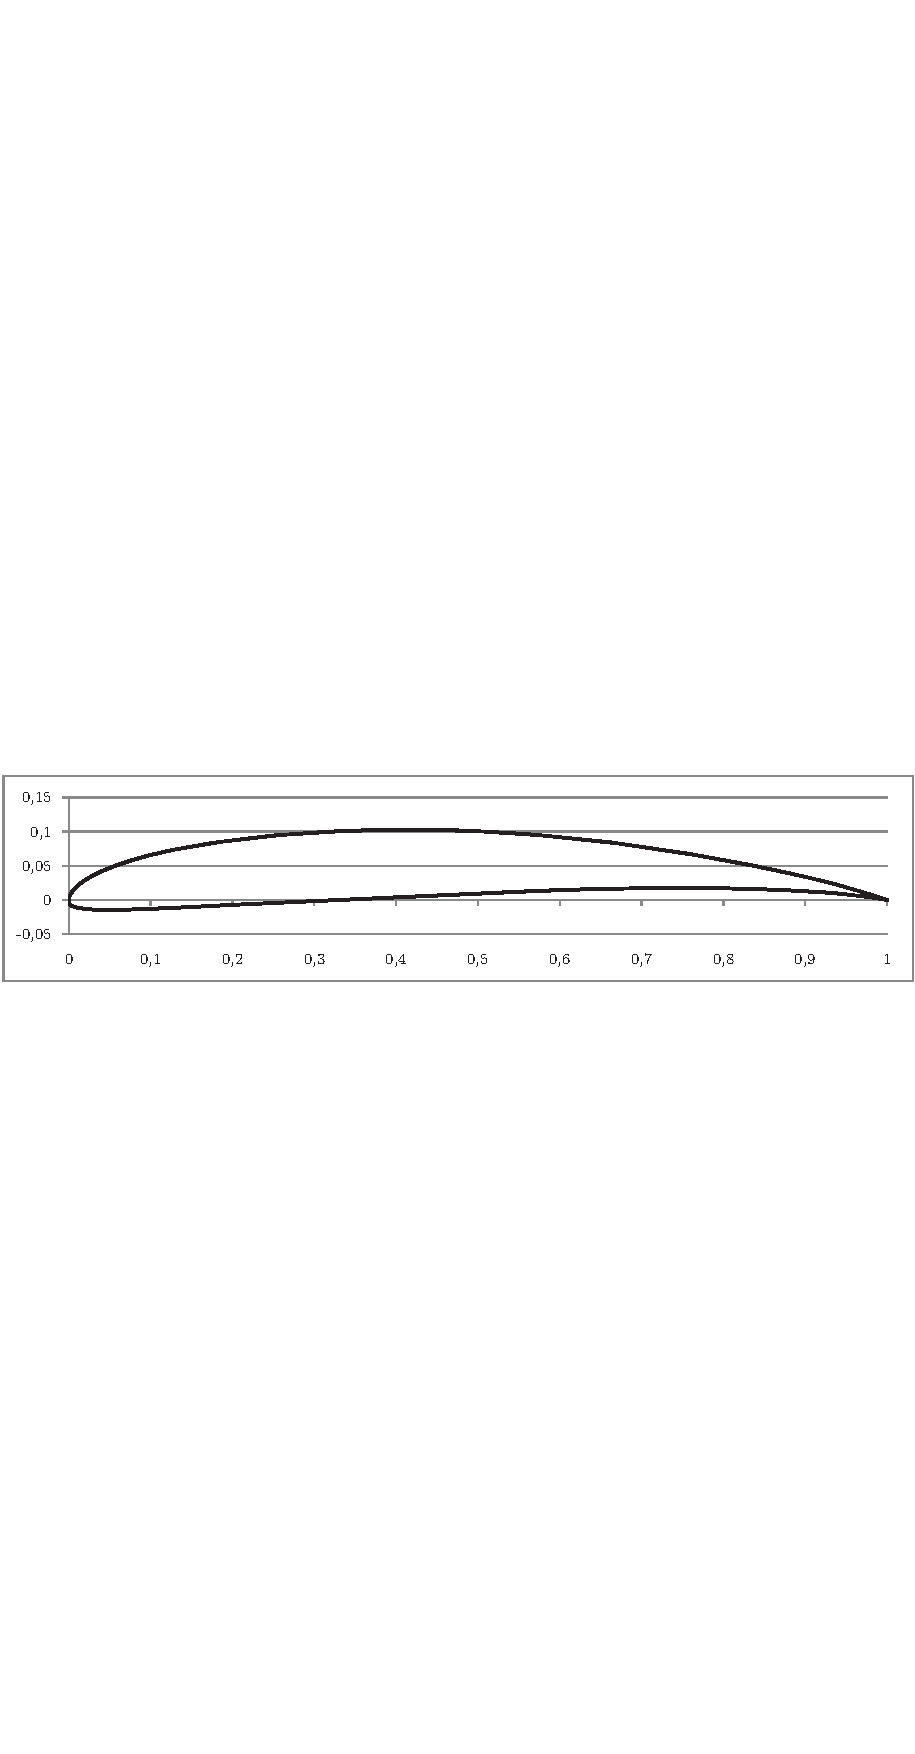
\includegraphics[]{obrazky/grafy/sgp}
				\caption{Profil SG6043}
				\label{profil:sg}
			\end{figure}
			\begin{figure}[H]
					\centering
					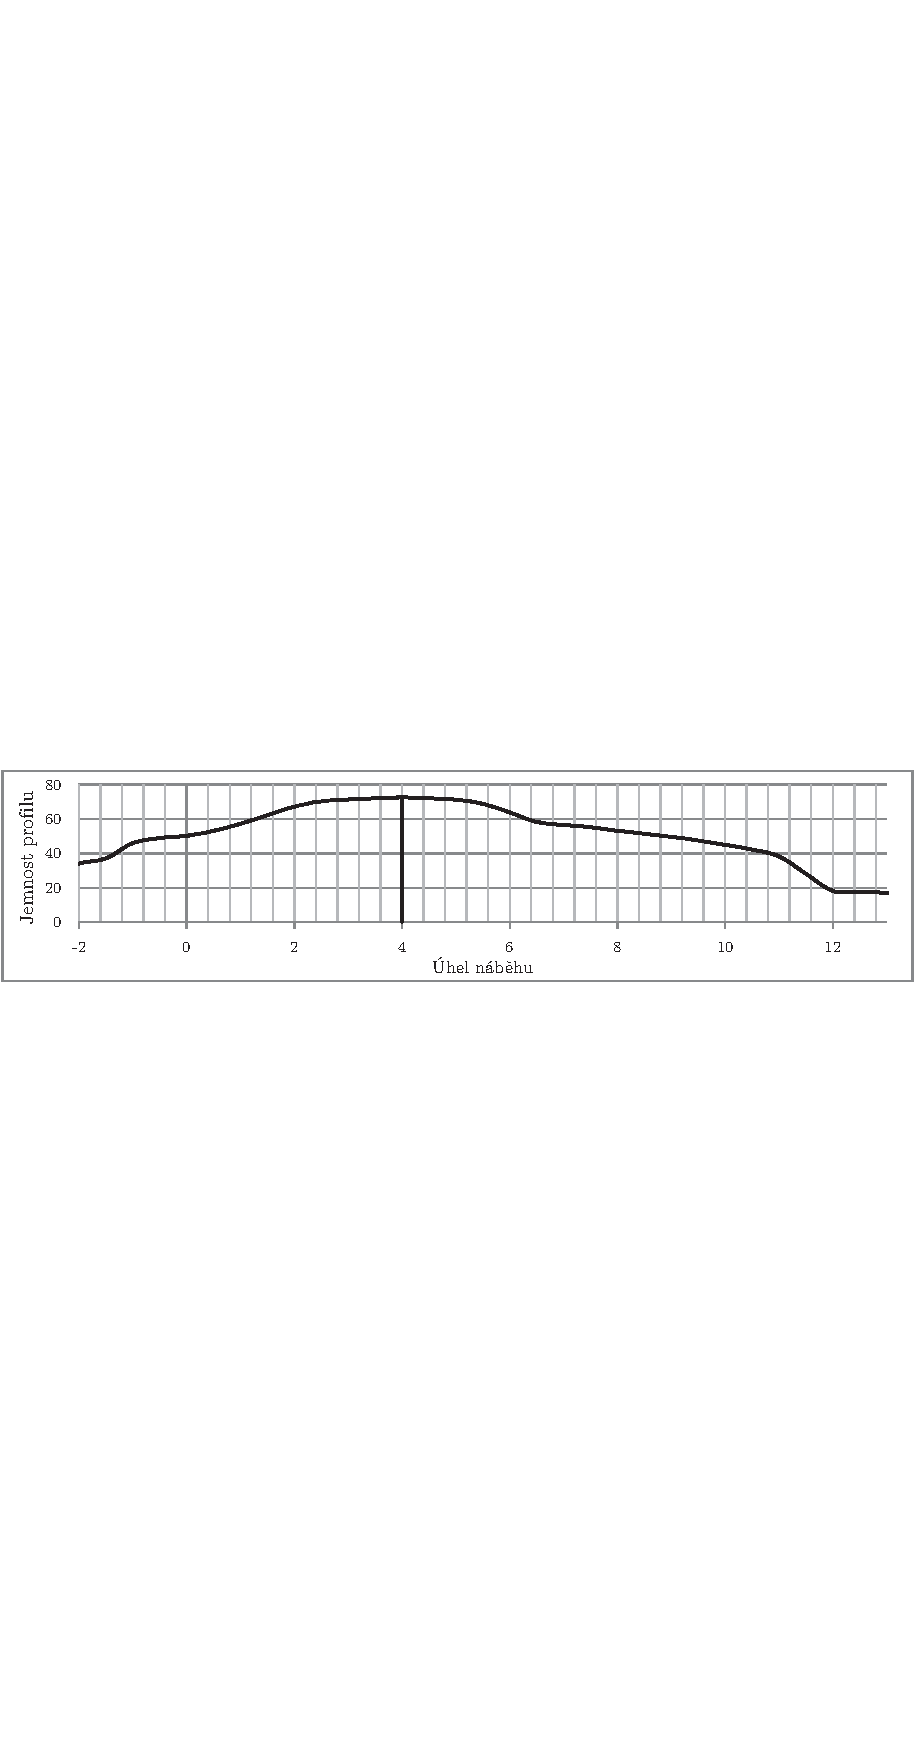
\includegraphics[]{obrazky/grafy/sgjp}
					\caption{Jemnost profilu SG6043}
					\label{profil:sgj}
			\end{figure}
	
	Z těchto profilů se ukázaly jako vhodné pouze 2; a to GOE481A a SG6043. Po zvážení jsem se rozhodl pro SG6043. Jednak má plynulejší průběh jemnosti a navíc s~ním mám už předchozí pozitivní zkušenosti
	
	\section{Postup výpočtu}\label{postup}
	V kapitole \ref{kap:funkce2} jsem zmínil, že výpočet podle Glauerta nelze řešit klasicky. V této kapitole bych rád vysvětlil jednak proč jej nelze řešit klasicky, ale hlavně také jak jej vyřešit.
	
	Při prvním pohledu na problematiku si lze všimnou koeficientů $h$ a $k$, které nejsou nějak definovány. Vystupují jako vstupní hodnota. Tyto koeficienty mohou nebývat nekonečně mnoha platných hodnot. Nás však zajímá hodnota, pro kterou dávají maximální výkon. Je proto vhodné zavést tzv. součinitel výkonu $C_p$ \eqref{rov:51}, který charakterizuje účinnost elementu turbíny na daném poloměru \cite{Rychetnik:Motory}.
	\begin{equation}
		\label{rov:51}
		C_p=\frac{\mathrm{d}P_{turbíny}}{\mathrm{d}P_{vzduchu}}=\frac{\omega\;\mathrm{d}M}{\rho\pi r \; \mathrm{d}rv_1^3}=\frac{\omega^2r^2(1+k)(h-1)}{v_1^2}=\lambda_r^2(1+k)(h-1)
	\end{equation}
	Z této definice by se mohlo zdát, že maximální výkon je nekonečně velký, nesmíme však zapomínat, že součinitelé $k$ a $h$ mají mezi sebou vztah. Tento vztah vychází z~výpočtu úhlu $\beta$ (rovnice \eqref{rov:36}). Pokud tento vztah dosadíme do výsledné rovnice teorie podle Glauerta (rovnice \eqref{rov:49}), získáme vztah \eqref{rov:52}.
		\begin{equation}
			\label{rov:52}
			k= 1 - \lambda_r(h-1)\cot(\beta-\varepsilon)
		\end{equation}
	Z těchto vztahů je patrná cyklická závislost – např. $\beta$ závisí na $k$ a $h$, přičemž $k$ závisí na $\beta$. Koeficient $k$ vychází z~neznámého koeficientu $h$ atd.
	
	Výpočet této soustavy lze provést pouze iteračně. Ručně je takovýto výpočet prakticky neproveditelný, ale na počítači je to otázka zlomků sekund.
	
	Než popíši postup výpočtu, rád bych zmínil ještě jeden poznatek patrný z výše uvedených vztahů. Koeficienty, potažmo i výkonový součinitel, vychází z~rychloběžnosti na poloměru $r$, nikoliv z~rychloběžnosti na konci lopatek. Tudíž budou tyto koeficienty na různých poloměrech různé. Z~tohoto poznatku také plyne to, že nelze sestavit parametrickou rovnici např. pro délku tětivy v~závislosti na poloměru, která by šla zadat přímo do CAD programu. Jednotlivé body této rovnice se totiž opět musí počítat iteračně.
	
	Postup výpočtu jsem zvolil následující. Z rovnice \eqref{rov:51} vyplývá, že $h > 1$, protože proud vzduchu je zpomalován, nikoliv urychlován (tedy $k > 0$) a součinitel výkonu musí být kladný. Pro výpočet je nutné odhadnou výchozí hodnoty. Pro koeficient $k$ jsem vybral výchozí hodnotu $\frac{1}{3}$ podle Betzovy účinnosti. Jelikož jsem se rozhodl iterovat podle $h$, zvolil jsem hodnotu blízkou~1, která je dostatečné malá, aby mohla dále růst a nebyla za maximem součinitele výkonu. Konkrétně $1 + 10^{-5}$.
	
	Z těchto koeficientů vypočítám podle rovnice \eqref{rov:36} úhel $\beta$. Následuje první krok iterace, kdy z~vypočteného úhlu vypočítám podle rovnice \eqref{rov:52} novou hodnotu koeficientu $k$. Z této hodnoty opět vypočítám úhel $\beta$, a tak dále. Tento výpočet opakuji tak dlouho, dokud není rozdíl dvou po sobě jdoucích výsledků menší, než zadaná přesnost.
	
	Až získám přesné hodnoty koeficientu $k$ a úhlu $\beta$ pro danou hodnotu koeficientu $h$, vypočtu součinitel výkonu. Pokud je větší než předchozí, inkrementuji koeficient $h$ o daný inkrement. Pokud je vypočtená hodnota menší, snížím koeficient $h$ o daný inkrement. Pokud má změna součinitele výkonu opačný směr než předcházející, snížím hodnotu inkrementu. Poté znovu začnu určovat hodnotu úhlu $\beta$ a koeficientu $k$, tentokrát však pro novou hodnotu $h$.
	
	Tento postup opakuji do té doby, než inkrement klesne pod zadanou hodnotu (přesnost výpočtu).
	
	Na provedení tohoto výpočtu jsem napsal jednoduchý konzolový program v jazyce C++. Bylo by jej možné napsat i v jiných jazycích, ale C++ je mi nejbližší. Zdrojový kód programu je přiložen v příloze (program je však rozšířen o další funkcionalitu – viz dále). Program byl zamýšlen jako jednoúčelový, na jedno použití. Z toho důvodu program nepřebírá žádný uživatelský vstup a veškerá vstupní data jsou zadávána přímo do zdrojového kódu.
	
	\section{Tvorba CAD modelu}\label{kap:model}
	Předchozí kapitoly shrnují, jak zjistit jednotlivé parametry turbíny, ale neposkytují informace o jejich použití. Tato kapitola popisuje, jak jsem ze získaných dat sestavil základní CAD model turbíny.
	
	CAD model jsem vytvořil v programu SolidWorks, jehož studentskou verzi používám. Model by šel obdobně vytvořit~i~v~ostatních programech.
	
	Základní model jsem vytvořil pomocí funkce \uv{přidat tažením po křivce}, kde jsem táhl aerodynamický profil po přímce za pomoci dvou vodících křivek – jedna běží po náběžné hraně, druhá běží po odtokové hraně.
	
	Z grafů \ref{graf.glauert1} a \ref{graf.glauert2} vyplývá, že křivka není žádnou \uv{běžnou} – nejedná se kružnici, parabolu, či hyperbolu. Pro křivku také dle předchozí kapitoly není možné sestavit parametrickou rovnici, která by se dala přímo zadat do SolidWorks. Jedinou možností je pro tuto křivku určit dostatečné množství bodů a naimportovat ji do SolidWorks. Ten z~těchto bodů následně křivku pomocí splajnu zrekonstruuje.
	
	Pro generování bodů křivky jsem upravil program zmíněný v předchozí kapitole. Program generuje textový sobor, kde jsou tabulátorem oddělené hodnoty zarovnané do sloupců. Tento formát jsem zvolil pro jeho širokou podporu – dá se přímo importovat jak do SolidWorks, tak i~např. do Microsoft Excelu a jiných.
	
	Prvním krokem bylo určení orientace listu v prostoru. Abych respektoval předvolené názvy základních rovin v SolidWorks (přední, pravá a horní), je list umístěn následovně. Z počátku souřadnic, ve směru osy X, vybíhá poloměr. Profil listu je umístěn v rovině YZ, s tím, že osa Y je umístěna proti směru větru.
	
	\begin{figure}[H]
			\centering
			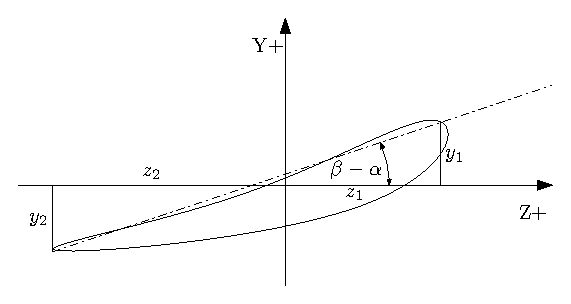
\includegraphics[]{obrazky/profilvprostoru}
			\caption{Umístění profilu v souřadném systému CAD programu.}
			\label{obr.profilosy}
		\end{figure}
	Z obrázku \ref{obr.profilosy} je patrné, jak lze spočítat souřadnice křivky pro náběžnou a odtokovou hranu. Náběžná hrana je křivka s body ve formátu [$r$, $y_1$, $z_1$], odtoková pak [$r$, $y_2$, $z_2$]. Výpočet těchto vzdáleností ukazují vztahy \eqref{rov:53}.
	\begin{eqnarray}
		\label{rov:53}
		y_1=bq\sin(\beta-\alpha) \nonumber \\
		z_1=bq\cos(\beta-\alpha) \nonumber \\
		y_2=b(q-1)\sin(\beta-\alpha)\nonumber \\
		z_2=b(q-1)\cos(\beta-\alpha)
	\end{eqnarray}
	Kde $b$ je délka tětivy, $\beta$ je úhel, který svírá směr relativního proud vzduchu s rovinou rotoru, $\alpha$ je úhel optimálního náběhu daného profilu a $q$ je koeficient vzdálenosti, ve které má profil největší tloušťku. Ten je zde proto, aby se profil v průběhu listu otáčel v místě s největší tloušťkou – cílem je získat co nejvíce prostoru na nosník.
	
	Tato úvaha však má jeden nedostatek – bod, okolo kterého se profil otáčí, neleží uprostřed profilu, ale na jeho tlakové hraně. Je proto nutné ho posunout o polovinu tloušťky profilu ve směru kolmém na tětivu. Tato úprava vypadá následovně\eqref{rov:54}.
	
	\begin{eqnarray}
		\label{rov:54}
		y_1=bq\sin(\beta-\alpha)+\frac{1}{2}bt\cos(\beta-\alpha) \nonumber \\
		z_1=bq\cos(\beta-\alpha)-\frac{1}{2}bt\sin(\beta-\alpha) \nonumber \\
		y_2=b(q-1)\sin(\beta-\alpha)+\frac{1}{2}bt\cos(\beta-\alpha)\nonumber \\
		y_2=b(q-1)\cos(\beta-\alpha)-\frac{1}{2}bt\sin(\beta-\alpha)
	\end{eqnarray}
	Kde $t$ je tloušťka profilu v~procentech délky tětivy profilu.
	Pro profil SG6043 je koeficient $q$~roven 0,33 a koeficient $t$~0,1 (patrno z tvaru tohoto profilu).  Použitím takto vypočtených křivek náběžné a odtokové hrany v prvku \uv{přidat tažením po křivce} vznikne následující model listu, potažmo celého rotoru (obrázky \ref{obr.model1} až \ref{obr.model3}).
	
	\begin{figure}[H]
				\centering
				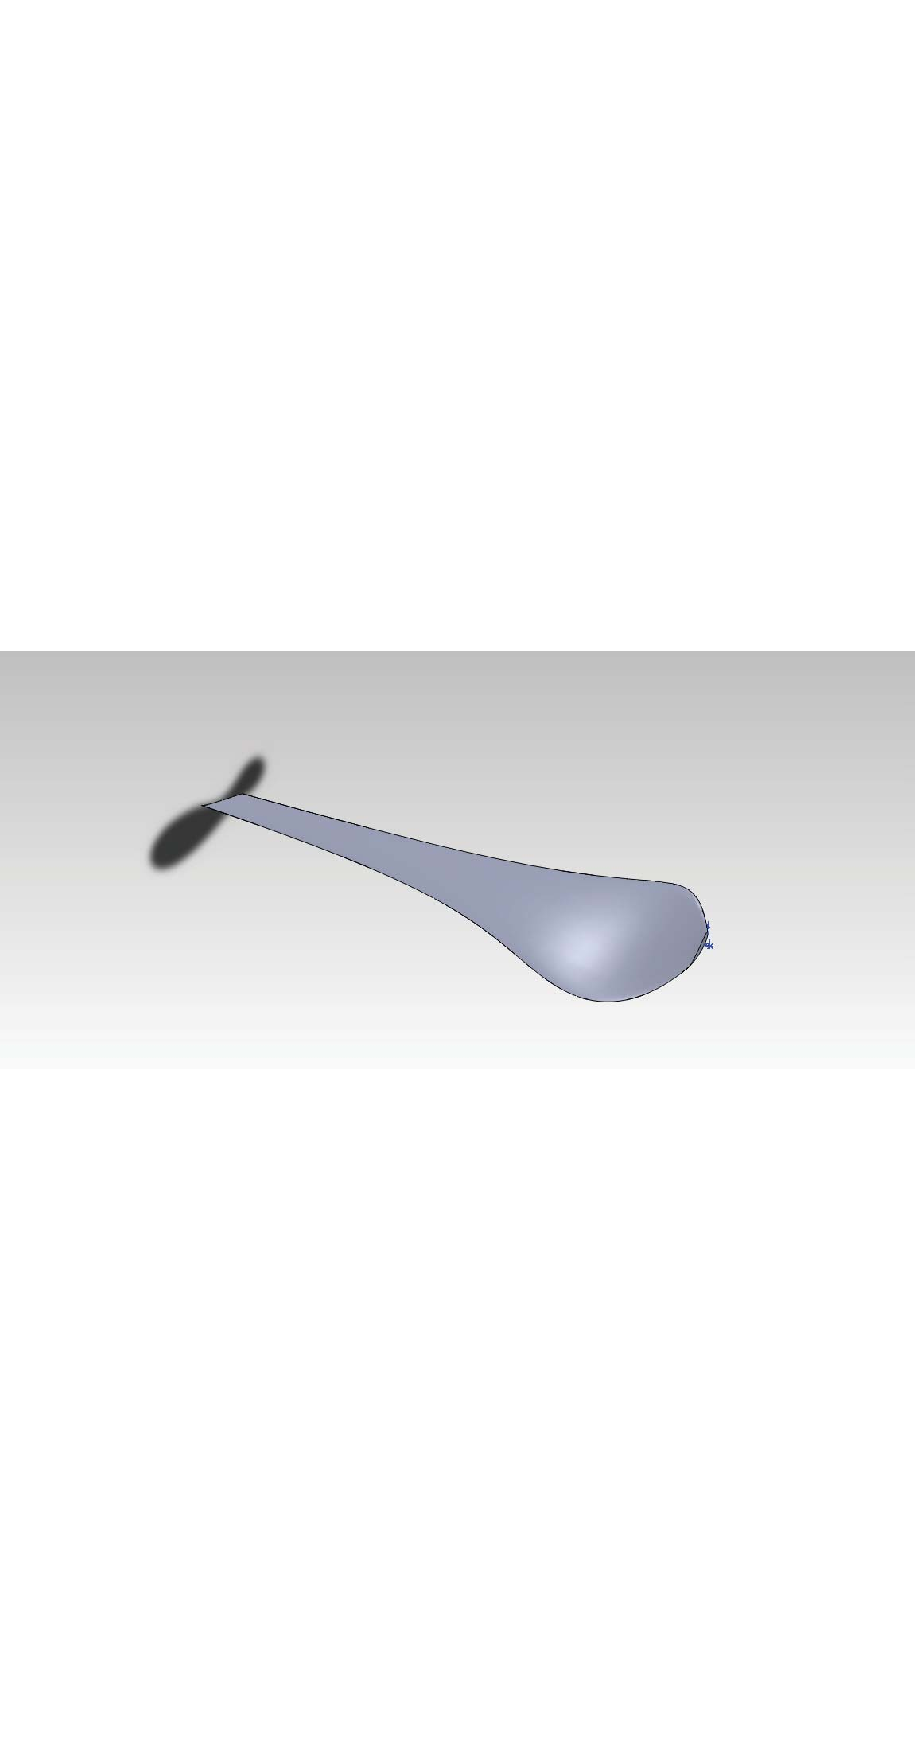
\includegraphics[]{obrazky/rotor/listp}
				\caption{Celkový pohled na rotorový list.}
				\label{obr.model1}
	\end{figure}
	
	\begin{figure}[H]
					\centering
					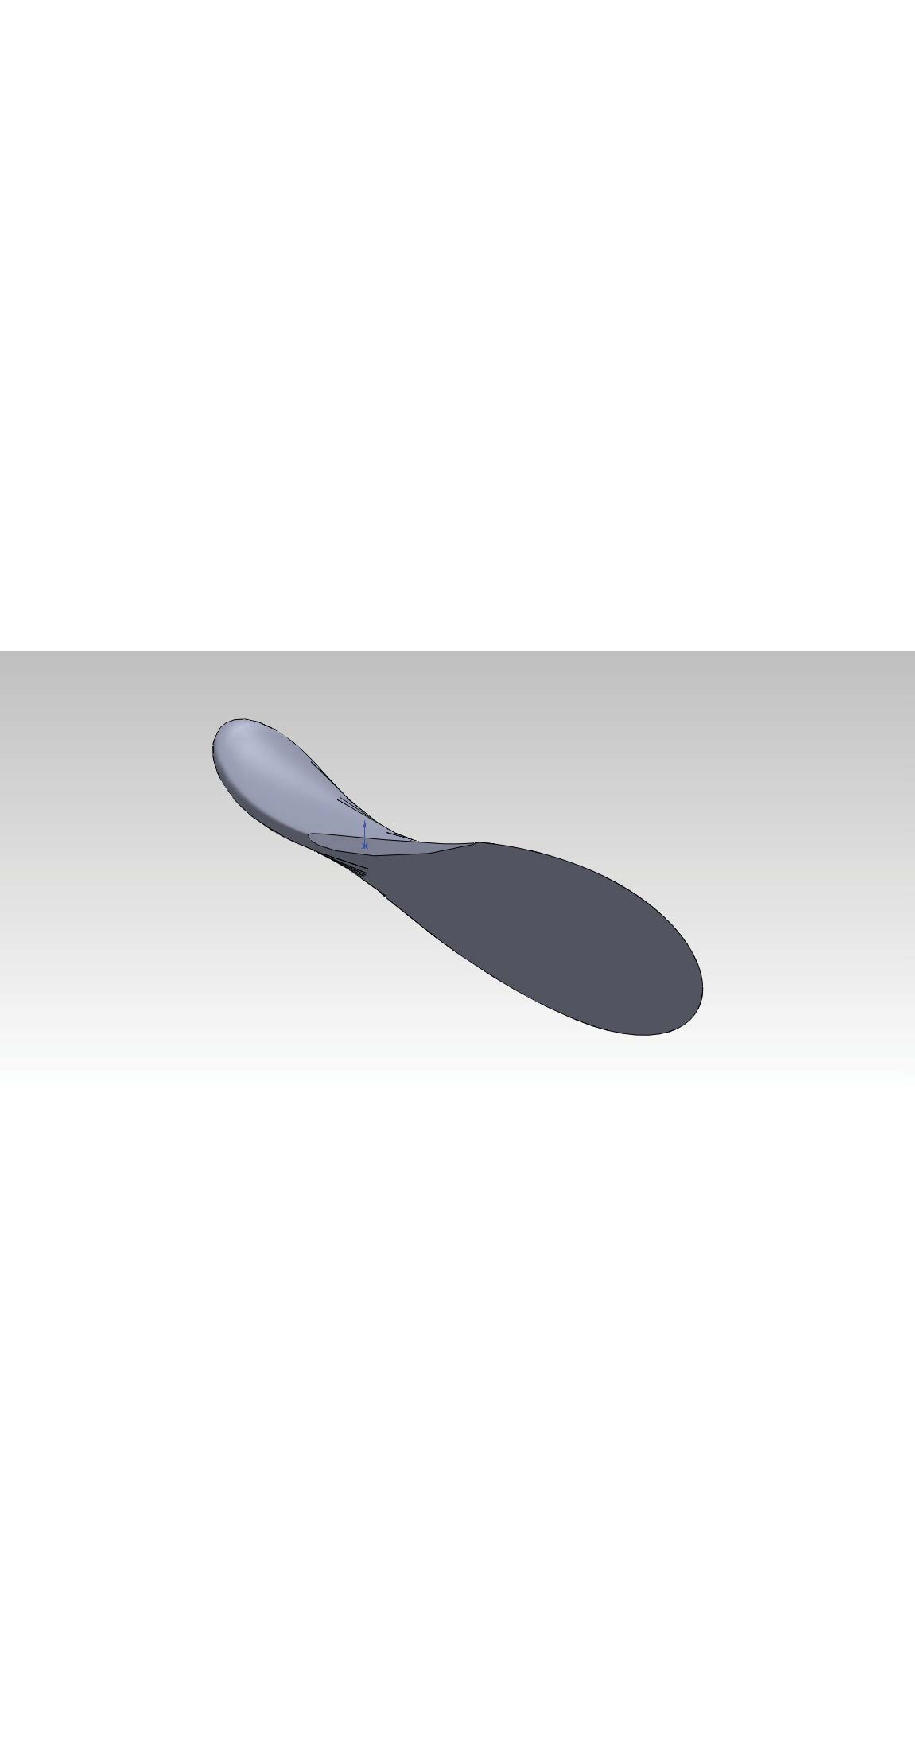
\includegraphics[]{obrazky/rotor/list2p}
					\caption{Pohled na list kolmo na pravou rovinu. Je zde patrný různý úhel náběhu a délka tětivy.}
					\label{obr.model2}
		\end{figure}
	\begin{figure}[H]
					\centering
					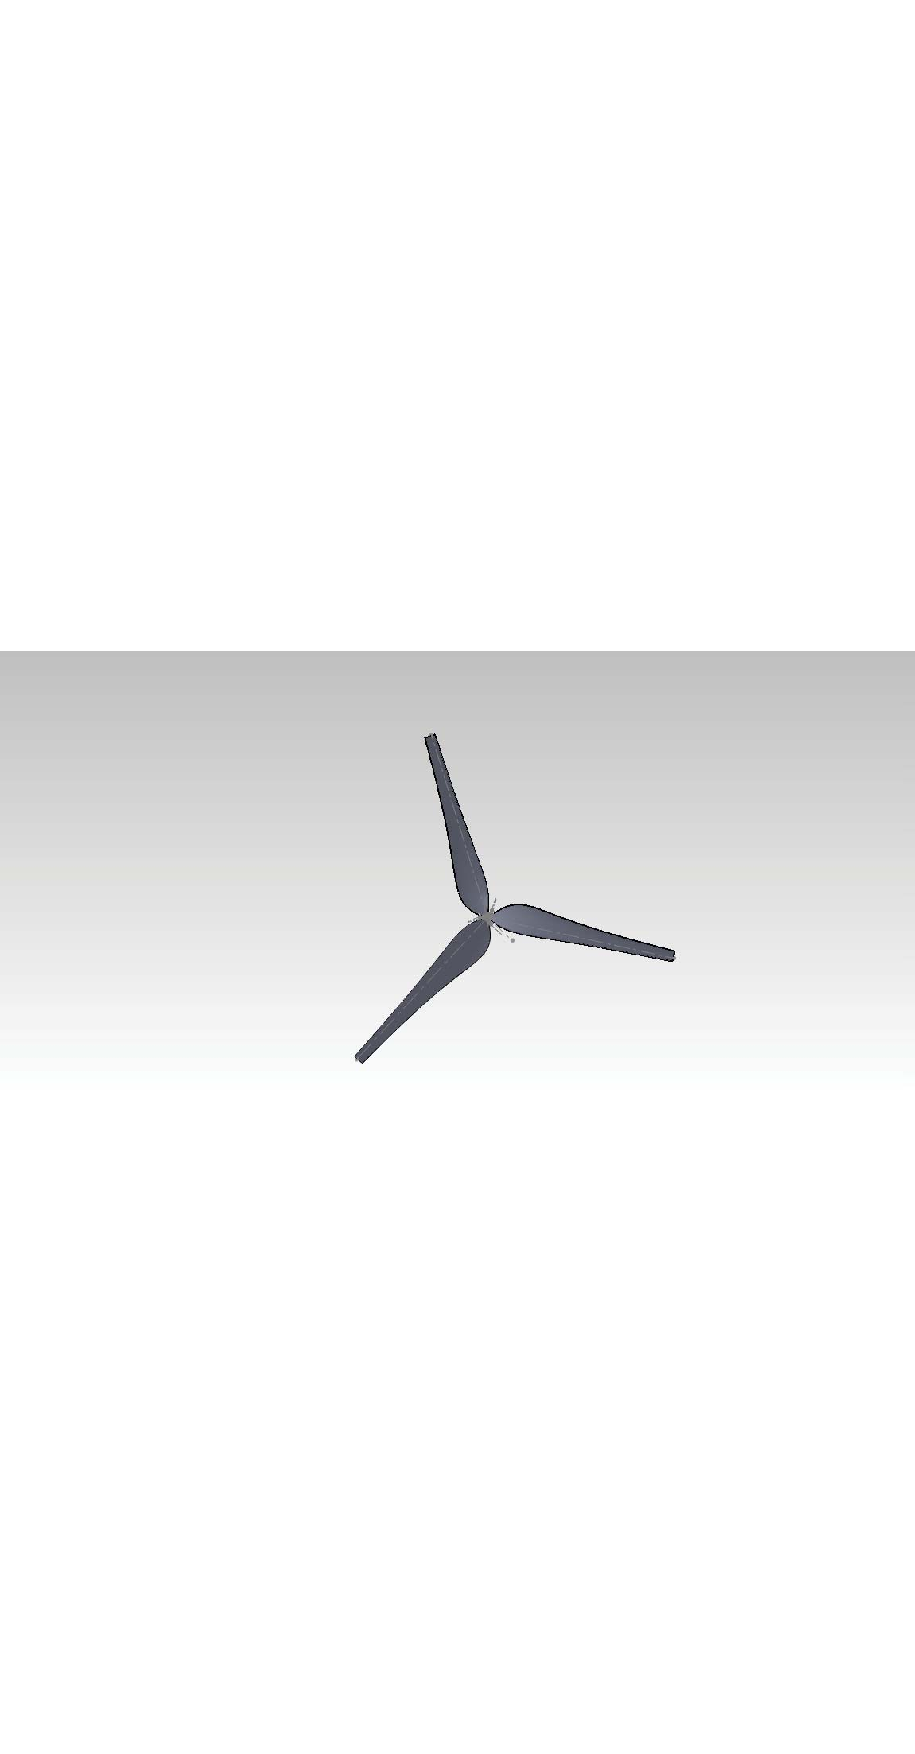
\includegraphics[]{obrazky/rotor/celekp}
					\caption{Pohled na celou turbínu složenou pouze ze 3 listů.}
					\label{obr.model3}
		\end{figure}
		
	\section{Parametry turbíny}
	Výše vytvořený model je teprve začátek návrhu. Potřebuje ještě několik úprav. Před jejich provedením bych však ještě rád uvedl parametry takto navržené turbíny.
	
	Data shrnuji v následujících třech tabulkách. Jsou vypočtena pro rychlosti větru 5~$m\cdot s^{-1}$ (tabulka \ref{tab:r5}), 10~$m\cdot s^{-1}$ (tabulka \ref{tab:r10}) a 25~$m\cdot s^{-1}$ (tabulka \ref{tab:r25}), což dle Beaufortovy stupnice odpovídá mírnému větru, čerstvému větru a vichřici.
	
	Data byla vypočtena pomocí tabulky v Microsoft Excelu pro jednotlivé elementy listu o~tloušťce 6,25~mm. Následně byly tyto hodnoty sečteny. Veškeré vztahy pro výpočet daných hodnot jsou uvedeny v kapitole \ref{kap:funkce2}. Hodnoty v~tabulkách jsou zaokrouhleny na celá čísla.
	\begin{table}[H]
		\centering
		\begin{tabular}{|l|l|}
		\hline
		Rychlost větru	&	5~$m\cdot s^{-1}$\\ \hline \hline
		Výkon vzduchu procházejícího turbínou	&441 $W$\\ \hline
		Axiální síla	&	69 $N$\\\hline
		Moment síly ohýbající list	&	32 $N\cdot m$\\\hline
		Síla roztáčející turbínu	&	15 $N$\\\hline
		Krouticí moment	&	11 $N\cdot m$\\\hline
		Otáčky rotoru	&	160 $min^{-1}$\\\hline
		Užitný výkon turbíny	&	176 $W$\\\hline	
		\end{tabular}
		\caption{Tabulka parametrů trurbíny pro rychlost 5~$m\cdot s^{-1}$}\label{tab:r5}
	\end{table}
	
		
		\begin{table}[H]
				\centering
				\begin{tabular}{|l|l|}
				\hline
				Rychlost větru	&	25~$m\cdot s^{-1}$\\ \hline \hline
				Výkon vzduchu procházejícího turbínou	&55 223 $W$\\ \hline
				Axiální síla	&1 734 $N$\\\hline
				Moment síly ohýbající list	&	481 $N\cdot m$\\\hline
				Síla roztáčející turbínu	&	390 $N$\\\hline
				Krouticí moment	&	262 $N\cdot m$\\\hline
				Otáčky rotoru	&	796 $min^{-1}$\\\hline
				Užitný výkon turbíny	&21 796 $W$\\\hline	
				\end{tabular}
				\caption{Tabulka parametrů trurbíny pro rychlost 25~$m\cdot s^{-1}$}\label{tab:r25}
			\end{table}
	
	Z těchto dat údajů si lze udělat představu jednak o podávaném výkonu a účinnosti, ale také hlavně o technických požadavcích na celou konstrukci. Je důležité si povšimnout, jak velká je síla působící na uložení, tedy i na stožár, a jak prudce roste. Stejně tak roste síla, která působí na list a ohýbá ho, potažmo ho vylamuje~z uložení v náboji. Všechny tyto parametry rostou s~třetí mocninou rychlosti větru. Důležité je uvažovat i působení odstředivé síly na listy, která roste \uv{pouze} s~druhou mocninou rychlosti větru. Tu však nelze spočítat, jelikož není známa konstrukce, a tudíž i hmotnost listu.
	
	Z těchto tabulek také vyplývá fakt, že turbína nutně potřebuje regulační zařízení, které ji při silném větru odstaví z~provozu. Reálný a bezpečný provoz je možný pouze pro rychlosti větru do 10–13~$m\cdot s^{-1}$.
	